\documentclass[tikz, border=20pt]{standalone}
\usepackage{tikz}
\usetikzlibrary{positioning, fit, calc, arrows.meta, backgrounds}

\begin{document}
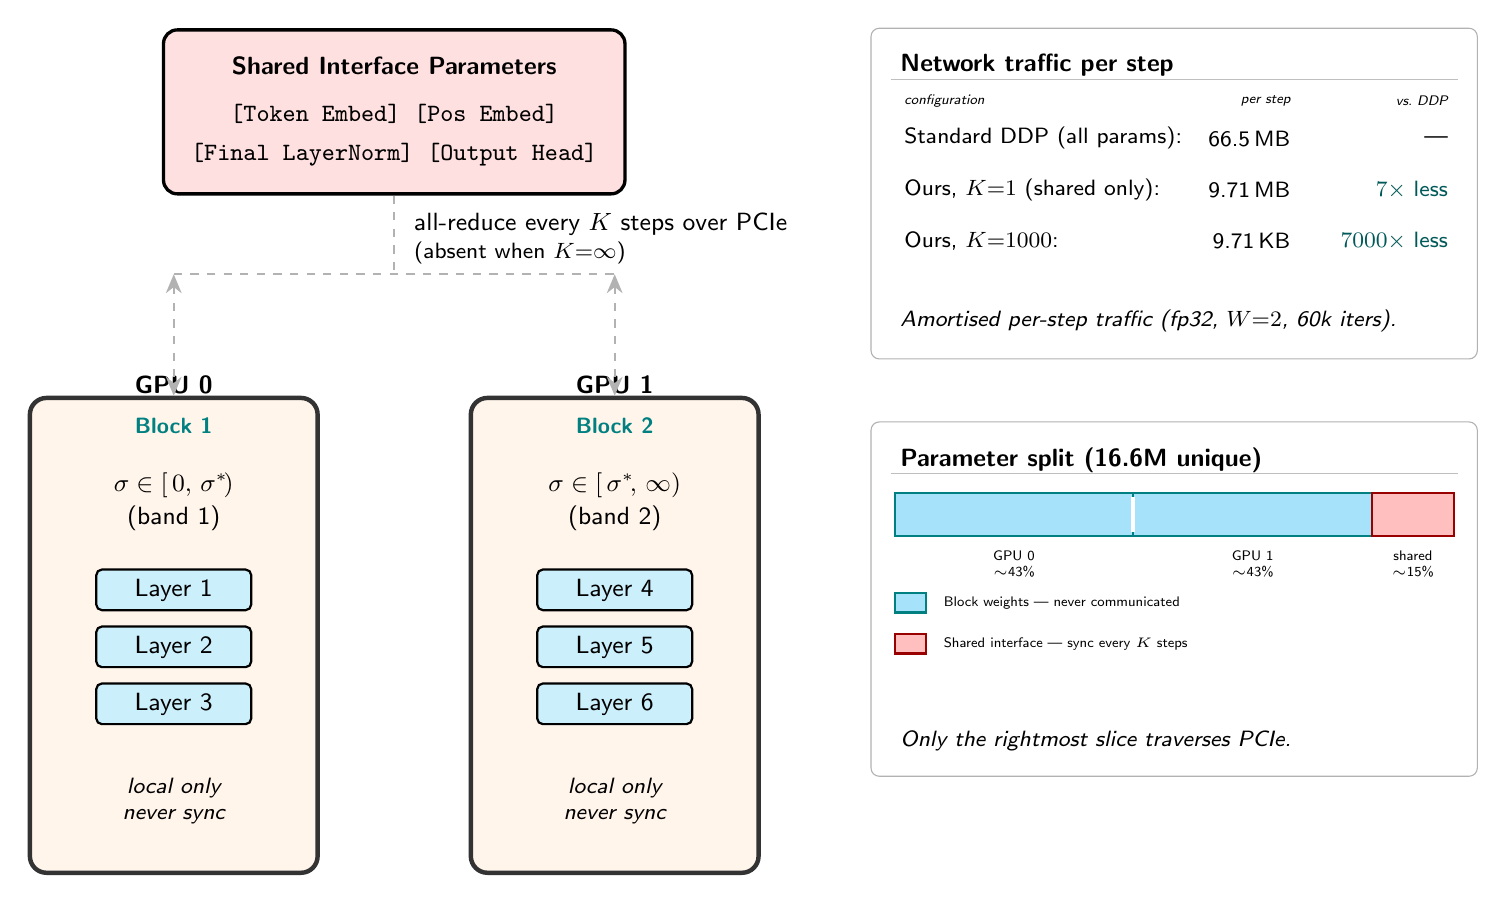
\begin{tikzpicture}[
  font=\sffamily,
  node distance=0.38cm,
  layernode/.style={
    draw, thick, rounded corners=2pt,
    fill=cyan!20, minimum width=13ex, minimum height=3.4ex,
    align=center, font=\small\sffamily
  },
  ifacebox/.style={
    draw, very thick, rounded corners=5pt,
    fill=red!12, inner sep=10pt, align=center
  },
  blockfit/.style={
    draw=teal, very thick, rounded corners=4pt,
    fill=cyan!6, inner sep=9pt
  },
  gpufit/.style={
    draw=black!80, ultra thick, rounded corners=6pt,
    fill=orange!8, inner sep=14pt
  },
  syncarrow/.style={
    {Stealth[length=2.4mm,width=2mm]}-{Stealth[length=2.4mm,width=2mm]},
    thick, dashed, gray!60
  },
  plainline/.style={thick, dashed, gray!60},
  insetbox/.style={draw=black!30, thin, rounded corners=3pt, fill=white},
]

%% ════════════════════════════════════════════════════════════════
%% LEFT: GPU diagram
%% ════════════════════════════════════════════════════════════════

%% ── Shared interface box ──────────────────────────────────────────
\node[ifacebox] (iface) {
  {\small\bfseries Shared Interface Parameters}\\[5pt]
  \texttt{\small[Token Embed]}\enspace\texttt{\small[Pos Embed]}\\[2pt]
  \texttt{\small[Final LayerNorm]}\enspace\texttt{\small[Output Head]}
};

%% ── GPU 0 ─────────────────────────────────────────────────────────
\node[below=3.4cm of iface, xshift=-2.8cm,
      font=\small\sffamily, align=center] (g0sigma)
  {$\sigma \in [\,0,\,\sigma^*\!)$\\[1pt](band 1)};
\node[layernode, below=0.35cm of g0sigma] (g0l1) {Layer 1};
\node[layernode, below=0.18cm of g0l1]    (g0l2) {Layer 2};
\node[layernode, below=0.18cm of g0l2]    (g0l3) {Layer 3};
\node[below=0.55cm of g0l3,
      font=\footnotesize\itshape\sffamily, align=center]
  (g0foot) {local only\\never sync};

\begin{pgfonlayer}{background}
  \node[blockfit, fit={(g0sigma)(g0l1)(g0l2)(g0l3)}] (block0) {};
  \node[gpufit,   fit={(block0)(g0foot)}]             (gpu0)   {};
\end{pgfonlayer}
\node[font=\footnotesize\bfseries\sffamily, text=teal]
  at ($(block0.north)+(0,4pt)$) {Block 1};
\node[font=\small\bfseries\sffamily]
  at ($(gpu0.north)+(0,4pt)$) {GPU~0};

%% ── GPU 1 ─────────────────────────────────────────────────────────
\node[below=3.4cm of iface, xshift=+2.8cm,
      font=\small\sffamily, align=center] (g1sigma)
  {$\sigma \in [\,\sigma^*\!,\,\infty)$\\[1pt](band 2)};
\node[layernode, below=0.35cm of g1sigma] (g1l4) {Layer 4};
\node[layernode, below=0.18cm of g1l4]    (g1l5) {Layer 5};
\node[layernode, below=0.18cm of g1l5]    (g1l6) {Layer 6};
\node[below=0.55cm of g1l6,
      font=\footnotesize\itshape\sffamily, align=center]
  (g1foot) {local only\\never sync};

\begin{pgfonlayer}{background}
  \node[blockfit, fit={(g1sigma)(g1l4)(g1l5)(g1l6)}] (block1) {};
  \node[gpufit,   fit={(block1)(g1foot)}]             (gpu1)   {};
\end{pgfonlayer}
\node[font=\footnotesize\bfseries\sffamily, text=teal]
  at ($(block1.north)+(0,4pt)$) {Block 2};
\node[font=\small\bfseries\sffamily]
  at ($(gpu1.north)+(0,4pt)$) {GPU~1};

%% ── Sync arrows ───────────────────────────────────────────────────
\coordinate (junction) at ($(iface.south)+(0,-1.0)$);
\coordinate (jl) at (junction -| gpu0.north);
\coordinate (jr) at (junction -| gpu1.north);

\draw[plainline] (iface.south) -- (junction);
\draw[plainline] (jl) -- (jr);
\draw[syncarrow] (jl) -- (gpu0.north);
\draw[syncarrow] (jr) -- (gpu1.north);

\node[font=\small\sffamily, align=left, fill=white,
      inner sep=2pt, rounded corners=2pt]
  at ($(iface.south)!0.55!(junction)+(5pt,0)$) [right]
  {all-reduce every $K$ steps over PCIe\\[-1pt]
   {\footnotesize (absent when $K{=}\infty$)}};


%% ════════════════════════════════════════════════════════════════
%% RIGHT COLUMN: stacked insets
%% x = gpu1.east + gap; y = iface.north (top of diagram)
%% ════════════════════════════════════════════════════════════════
\coordinate (rcx) at ($(gpu1.east)+(1.4, 0)$);
\coordinate (rc)  at (rcx |- iface.north);

%% Box dimensions
\pgfmathsetmacro{\RW}{7.7}    % right column width (cm)
\pgfmathsetmacro{\TH}{4.2}    % traffic box height
\pgfmathsetmacro{\PH}{4.5}    % param box height

%% ── TOP-RIGHT: Network traffic per step ──────────────────────────
\begin{scope}[shift={(rc)}]

  \draw[insetbox] (0,-\TH) rectangle (\RW, 0);

  %% title
  \node[font=\small\bfseries\sffamily, anchor=north west]
    at (0.25,-0.20) {Network traffic per step};

  %% separator
  \draw[black!25, thin] (0.25,-0.65) -- (7.45,-0.65);

  %% col headers
  \node[font=\tiny\sffamily\itshape, anchor=west]  at (0.30,-0.92) {configuration};
  \node[font=\tiny\sffamily\itshape, anchor=east]  at (5.45,-0.92) {per step};
  \node[font=\tiny\sffamily\itshape, anchor=east]  at (7.45,-0.92) {vs.\ DDP};

  %% row 1: DDP
  \node[font=\footnotesize\sffamily, anchor=west]  at (0.30,-1.40) {Standard DDP (all params):};
  \node[font=\footnotesize\sffamily, anchor=east]  at (5.45,-1.40) {66.5\,MB};
  \node[font=\footnotesize\sffamily, anchor=east]  at (7.45,-1.40) {—};

  %% row 2: K=1
  \node[font=\footnotesize\sffamily, anchor=west]  at (0.30,-2.05) {Ours, $K{=}1$ (shared only):};
  \node[font=\footnotesize\sffamily, anchor=east]  at (5.45,-2.05) {9.71\,MB};
  \node[font=\footnotesize\sffamily, anchor=east, text=teal!70!black]
    at (7.45,-2.05) {$7{\times}$ less};

  %% row 3: K=1000
  \node[font=\footnotesize\sffamily, anchor=west]  at (0.30,-2.70) {Ours, $K{=}1000$:};
  \node[font=\footnotesize\sffamily, anchor=east]  at (5.45,-2.70) {9.71\,KB};
  \node[font=\footnotesize\sffamily, anchor=east, text=teal!70!black]
    at (7.45,-2.70) {$7000{\times}$ less};

  %% caption
  \node[font=\footnotesize\itshape\sffamily, anchor=north west, text width=7.2cm]
    at (0.25,-3.45) {Amortised per-step traffic (fp32, $W{=}2$, 60k iters).};

\end{scope}

%% ── BOTTOM-RIGHT: Parameter split ────────────────────────────────
%% 16.6M unique params; wte tied to lm_head — communicated once, not twice.
%%   Block params: 14.2M = 85.4%  (split equally: 42.7% per GPU)
%%   Shared iface:  2.4M = 14.6%  (wte+wpe+ln_f; lm_head = wte, 1 tensor)
%%
%% Hardcoded offset from rc so gap is explicit and cannot drift.
\coordinate (rc2) at ($(rc)+(0,-5.0)$);

\pgfmathsetmacro{\barW}{\RW-0.6}
\pgfmathsetmacro{\barH}{0.55}
\pgfmathsetmacro{\bxA}{0.3}
\pgfmathsetmacro{\bxD}{\bxA+\barW}
\pgfmathsetmacro{\bxB}{\bxA + 0.427*\barW}
\pgfmathsetmacro{\bxC}{\bxB + 0.427*\barW}

\begin{scope}[shift={(rc2)}]

  \draw[insetbox] (0,-\PH) rectangle (\RW, 0);

  %% title
  \node[font=\small\bfseries\sffamily, anchor=north west]
    at (0.25,-0.20) {Parameter split (16.6M unique)};

  %% separator
  \draw[black!25, thin] (0.25,-0.65) -- (7.45,-0.65);

  %% bar (top at y=-0.90)
  \pgfmathsetmacro{\bY}{-0.90}
  \fill[cyan!35, draw=teal, thick]
    (\bxA,{\bY-\barH}) rectangle (\bxB,\bY);
  \fill[cyan!35, draw=teal, thick]
    (\bxB,{\bY-\barH}) rectangle (\bxC,\bY);
  \draw[white, line width=1.5pt]
    (\bxB,{\bY-\barH+0.05}) -- (\bxB,{\bY-0.05});
  \fill[red!25, draw=red!60!black, thick]
    (\bxC,{\bY-\barH}) rectangle (\bxD,\bY);

  %% labels below bar
  \node[font=\tiny\sffamily, align=center, anchor=north]
    at ({(\bxA+\bxB)/2},{\bY-\barH-0.06})
    {GPU 0\\$\sim$43\%};
  \node[font=\tiny\sffamily, align=center, anchor=north]
    at ({(\bxB+\bxC)/2},{\bY-\barH-0.06})
    {GPU 1\\$\sim$43\%};
  \node[font=\tiny\sffamily, align=center, anchor=north]
    at ({(\bxC+\bxD)/2},{\bY-\barH-0.06})
    {shared\\$\sim$15\%};

  %% legend rows
  \pgfmathsetmacro{\lY}{-2.50}
  \fill[cyan!35, draw=teal, thick]
    (0.30,{\lY+0.08}) rectangle (0.70,{\lY+0.33});
  \node[font=\tiny\sffamily, anchor=west] at (0.80,{\lY+0.20})
    {Block weights — never communicated};

  \pgfmathsetmacro{\lYb}{\lY-0.52}
  \fill[red!25, draw=red!60!black, thick]
    (0.30,{\lYb+0.08}) rectangle (0.70,{\lYb+0.33});
  \node[font=\tiny\sffamily, anchor=west] at (0.80,{\lYb+0.20})
    {Shared interface — sync every $K$ steps};

  %% caption
  \node[font=\footnotesize\itshape\sffamily, anchor=north west, text width=7.2cm]
    at (0.25,-3.80) {Only the rightmost slice traverses PCIe.};

\end{scope}

\end{tikzpicture}
\end{document}
